\chapter{Experiments and Evaluation}
\label{chap:experiments}

This chapter presents the empirical evaluation of DBMS-Nautilus, a grammar-based fuzzer for SQLite. The evaluation is organized around three research questions that address CVE rediscovery effectiveness, new bug detection capability, and performance trade-offs relative to the EBNF-Baseline. Section~\ref{sec:rqs} states the research questions. Section~\ref{sec:metrics} defines the evaluation metrics. Section~\ref{sec:baselines} introduces the baseline. Section~\ref{sec:setup} describes the experimental setup. Section~\ref{sec:results} presents the results. Section~\ref{sec:discussion} provides analysis and discussion.


\section{Research Questions}
\label{sec:rqs}

The evaluation addresses the following three research questions:

\begin{description}
  \item[RQ1 (CVE Rediscovery).] Can DBMS-Nautilus, augmented with low-weight seed rules, reliably rediscover known CVEs in historical SQLite versions?
  \item[RQ2 (New Bug Detection).] Does DBMS-Nautilus, without CVE-specific seed rules, discover previously unreported bug classes beyond the target CVEs?
  \item[RQ3 (Performance Trade-off).] How does DBMS-Nautilus compare to the EBNF-Baseline in terms of throughput, edge coverage, unique root causes, and time to first crash?
\end{description}

RQ1 measures targeted effectiveness: whether domain-knowledge-driven grammar engineering can reconstruct CVE-triggering inputs from independently encoded structural primitives. RQ2 evaluates generality: whether the same grammar discovers bugs that were not anticipated during grammar design, providing evidence for cross-pollination between structural patterns. RQ3 quantifies the cost of structural complexity: DBMS-Nautilus generates longer, more complex SQL inputs than a generic grammar, and this section measures whether the resulting throughput reduction is offset by improved bug-finding capability.





\section{Evaluation Metrics}
\label{sec:metrics}

Six metrics are used across the three research questions:

\begin{description}
  \item[\textbf{CVE rediscovery rate} (RQ1).] The proportion of target CVEs for which at least one crash matching the CVE's structural signature was observed across all campaign runs. A crash is classified as a CVE rediscovery if its stack trace matches the CVE signature library with at least 80\% fidelity, defined as the ratio of matching frames to total signature frames in the top 5 frames of the crashing call stack.

  \item[\textbf{Unique bug classes} (RQ2).] The number of distinct bug classes discovered, where each class is defined by the combination of the crashing function and the sanitizer diagnostic type (null pointer dereference, integer overflow, misaligned access, signal, or float cast overflow). Bug classes are identified through stack-hash deduplication using the top 5 frames of the crashing call stack, then grouped by key function.

  \item[\textbf{Unique root causes} (RQ3).] The number of unique stack hashes per campaign, computed from the top 5 frames of the crashing call stack after filtering system library and sanitizer runtime frames. This metric captures the diversity of crash-inducing inputs within a single campaign.

  \item[\textbf{Edge coverage} (RQ3).] The number of unique edges (branch transitions) recorded in the AFL-style coverage bitmap during a campaign. Edge coverage measures the breadth of code exploration and is formally defined as:
  \begin{equation}
    \text{EdgeCov}(C) = \left|\left\{ (b_i, b_j) \mid \exists\, t \in C : (b_i, b_j) \in \text{edges}(t) \right\}\right|
    \label{eq:edgecov}
  \end{equation}
  where $C$ is the set of test cases executed during the campaign, $b_i$ and $b_j$ are basic blocks, and $\text{edges}(t)$ is the set of branch transitions observed during execution of test case $t$.

  \item[\textbf{Throughput} (RQ3).] The number of test case executions per second, measuring the raw speed of the fuzzing campaign. Higher throughput allows more inputs to be tested within a fixed time budget, but does not guarantee better bug discovery if the generated inputs lack structural diversity.

  \item[\textbf{Time to first crash (TTFC)} (RQ3).] The wall-clock time from campaign start to the first test case that triggers a non-zero exit code from the harness. TTFC measures how quickly the fuzzer finds any crash-inducing input, regardless of whether the crash corresponds to a known CVE or a unique bug class.
\end{description}









\section{The EBNF-Baseline}
\label{sec:baselines}

The baseline for comparison is the EBNF-Baseline, a standard EBNF SQL grammar derived from SQLite's public grammar specification. This grammar defines all syntactically valid SQL statement types (\texttt{SELECT}, \texttt{INSERT}, \texttt{UPDATE}, \texttt{DELETE}, \texttt{CREATE}, \texttt{DROP}, \texttt{PRAGMA}, etc.) with uniform production rule weights and no domain-specific structural primitives, no CVE-motivated rules, and no weight tuning. It represents grammar-based fuzzing without domain knowledge --- the approach a practitioner would use when applying a grammar-based fuzzer to SQLite with only the language specification. The EBNF-Baseline uses the same pre-loaded schema and identical campaign parameters (15-minute duration, 300-node maximum tree size, 500\,ms timeout, single thread) as DBMS-Nautilus, ensuring that any performance difference is attributable solely to grammar design.

\textbf{DBMS-Nautilus} encodes domain-specific structural patterns extracted from CVE root-cause analysis as weighted production rules. It contains 526 production rules organized around four statement shapes, six schema templates, and eight query types, augmented with boundary-value terminals, window function patterns, self-referential generated column rules, compound query operators, and JSON/JSONB function rules. For RQ1, six low-weight seed rules are added to DBMS-Nautilus to ensure all target CVEs are within the grammar's generation range; for RQ2 and RQ3, the grammar is used without seed rules.




\section{Experimental Setup}
\label{sec:setup}

\subsection{Subjects Under Test}
\label{sec:subjects}

Four SQLite versions with confirmed CVEs served as the primary subjects under test, selected according to three criteria: (1)~\emph{popularity} --- SQLite is the most widely deployed database engine, embedded in virtually all mobile devices, web browsers, and operating systems; (2)~\emph{diversity} --- the four versions span two years of development (2019--2020) and contain four distinct CVEs covering integer overflow, null pointer dereference, use-after-free, and heap buffer overflow bug types; (3)~\emph{reproducibility} --- all versions are publicly available as amalgamation source files, and all target CVEs have published proof-of-concept inputs enabling independent verification.

Table~\ref{tab:subjects} summarizes the subjects under test. Each version was compiled from the SQLite amalgamation (a single C source file of approximately 150{,}000 lines) using Clang~14 with AddressSanitizer (ASan)~\citep{asan} and UndefinedBehaviorSanitizer (UBSan) instrumentation. Version~3.30.1 is included as a subject because CVE-2020-13434 affects versions 3.30.1 through 3.32.0 and CVE-2020-13871 was independently discovered on this version during evaluation.

\begin{table}[htbp]
\caption{Subjects under test.}
\label{tab:subjects}
\centering
\resizebox{\textwidth}{!}{%
\begin{tabular}{llll}
\toprule
\textbf{Version} & \textbf{Release} & \textbf{CVE(s)} & \textbf{Bug Type} \\
\midrule
3.30.1 & 2019-10 & CVE-2020-13434, CVE-2020-13871 & Int overflow, use-after-free \\
3.31.1 & 2020-01 & CVE-2020-13434 & Int overflow \\
3.32.0 & 2020-05 & CVE-2020-13434, CVE-2020-13435 & Int overflow, null ptr deref \\
3.32.2 & 2020-06 & CVE-2020-15358, CVE-2020-13871 & Heap overflow, use-after-free \\
\bottomrule
\end{tabular}}
\end{table}

\subsection{Environment and Campaign Configuration}
\label{sec:environment}

All experiments were conducted on a workstation equipped with an ARM-based processor (aarch64), 8~GB of RAM, and running Ubuntu 22.04 LTS. The fuzzer was compiled with Rust 1.93 in release mode. All SQLite harness binaries were compiled with Clang~14 using ASan and UBSan instrumentation, with the \texttt{-DSQLITE\_DEBUG} flag enabled for the primary fuzzing harnesses. Separate harness binaries without \texttt{SQLITE\_DEBUG} were built for CVE confirmation replay (see Section~\ref{sec:rq1-results}).



Table~\ref{tab:params} summarizes the campaign parameters. All campaigns used a 15-minute (900-second) duration with 5 independent repetitions per configuration, for a total of 79 campaigns across the three research questions (20 for RQ1, 20 for RQ2, and 39 for RQ3 --- 2 grammars $\times$ 4 versions $\times$ 5 runs; one EBNF-Baseline campaign on version 3.32.0 was excluded due to a missing workdir). A single fuzzing thread was used in all campaigns to eliminate concurrency-related variance and ensure reproducibility. The maximum tree size of 300 nodes limits the complexity of generated SQL statements, preventing excessively long inputs that would dominate execution time without contributing to coverage.

\begin{table}[htbp]
\caption{Campaign parameters.}
\label{tab:params}
\centering
\begin{tabular}{ll}
\toprule
\textbf{Parameter} & \textbf{Value} \\
\midrule
Campaign duration & 900 seconds (15 minutes) \\
Repetitions per configuration & 5 \\
Maximum tree size & 300 nodes \\
Execution timeout & 500 ms \\
Fuzzing threads & 1 \\
Coverage bitmap size & 2 MB (2{,}097{,}152 bytes) \\
\bottomrule
\end{tabular}
\end{table}





\section{Results}
\label{sec:results}

\subsection{RQ1: CVE Rediscovery}
\label{sec:rq1-results}

DBMS-Nautilus with seed rules was evaluated across all four SQLite versions (5 runs per version, 20 runs total). Table~\ref{tab:cve-rediscovery} presents the CVE rediscovery results.

\begin{table}[htbp]
\caption{CVE rediscovery results.}
\label{tab:cve-rediscovery}
\centering
\resizebox{\textwidth}{!}{%
\begin{tabular}{@{}l@{\hspace{8pt}}l@{\hspace{8pt}}l@{\hspace{8pt}}c@{\hspace{8pt}}c@{}}
\toprule
\textbf{CVE} & \textbf{Bug Type} & \textbf{Version(s)} & \textbf{DBMS-Nautilus} & \textbf{EBNF-Baseline} \\
\midrule
CVE-2020-13434 & Int overflow & 3.30.1, 3.31.1, 3.32.0 & \textbf{14/15} & 0/15 \\
CVE-2020-13435 & Null ptr deref & 3.32.0 & \textbf{5/5} & 0/5 \\
CVE-2020-13871 & Use-after-free & 3.30.1 & \textbf{4/5}\textsuperscript{*} & 4/5 \\
CVE-2020-15358 & Heap overflow & 3.32.2 & \textbf{5/5} & 0/5 \\
\midrule
\multicolumn{3}{@{}l}{\textbf{Total CVEs confirmed}} & \textbf{4/4} & \textbf{1/4} \\
\bottomrule
\end{tabular}}
\smallskip\noindent\textsuperscript{*}One run produced a stack trace below the 80\% fidelity threshold.
\end{table}

Table~\ref{tab:trigger-sql} compares the SQL inputs generated by DBMS-Nautilus with the original CVE proof-of-concept for each confirmed rediscovery. The generated inputs preserve the structural pattern of the original PoC while using the grammar's own table and column names from the pre-loaded schema.

\begin{table}[htbp]
\caption{Trigger SQL generated by DBMS-Nautilus vs original CVE proof-of-concept.}
\label{tab:trigger-sql}
\centering
\small
\begin{tabular}{lp{5.5cm}p{5.5cm}}
\toprule
\textbf{CVE} & \textbf{Original PoC} & \textbf{DBMS-Nautilus Trigger} \\
\midrule
CVE-2020-13434 &
\texttt{SELECT printf('\%.*g', 2147483647, 0.01);} &
\texttt{SELECT printf('\%.*g', -2147483649, 0.01);} \\
\addlinespace
CVE-2020-13435 &
\texttt{CREATE TABLE a(c UNIQUE); SELECT a.c FROM a JOIN a b ON 3 = a.c NATURAL JOIN a WHERE a.c IN(...);} &
\texttt{CREATE TABLE seed\_a(c UNIQUE); SELECT seed\_a.c FROM seed\_a JOIN seed\_a b ON 3 = seed\_a.c NATURAL JOIN seed\_a WHERE seed\_a.c IN(...);} \\
\addlinespace
CVE-2020-13871 &
\texttt{SELECT(SELECT b FROM a GROUP BY b HAVING(...)) FROM a EXCEPT SELECT b FROM a ORDER BY b;} &
\texttt{SELECT(SELECT b FROM seed\_b GROUP BY b HAVING(...)) FROM seed\_b EXCEPT SELECT b FROM seed\_b ORDER BY b;} \\
\addlinespace
CVE-2020-15358 &
\texttt{SELECT * FROM t1, t2 WHERE c1=(SELECT 123 INTERSECT SELECT c2 FROM t5);} &
\texttt{CREATE TABLE p(a DATE, b AS(b) UNIQUE); VALUES (...) INTERSECT VALUES (...); SELECT * FROM seed\_t1, seed\_t2 WHERE c1=(...);} \\
\bottomrule
\end{tabular}
\end{table}

DBMS-Nautilus confirmed 4 of 4 target CVEs, while the EBNF-Baseline found only CVE-2020-13871. The EBNF-Baseline's discovery of CVE-2020-13871 indicates that the window function code path is reachable through generic SQL generation.

Figure~\ref{fig:time-to-cve} compares the time to first CVE-matching crash between DBMS-Nautilus and the EBNF-Baseline. For the three CVEs that the EBNF-Baseline never found, the bars are shown at the full campaign duration (900\,s) with hatched fill.

\begin{figure}[htbp]
\centering
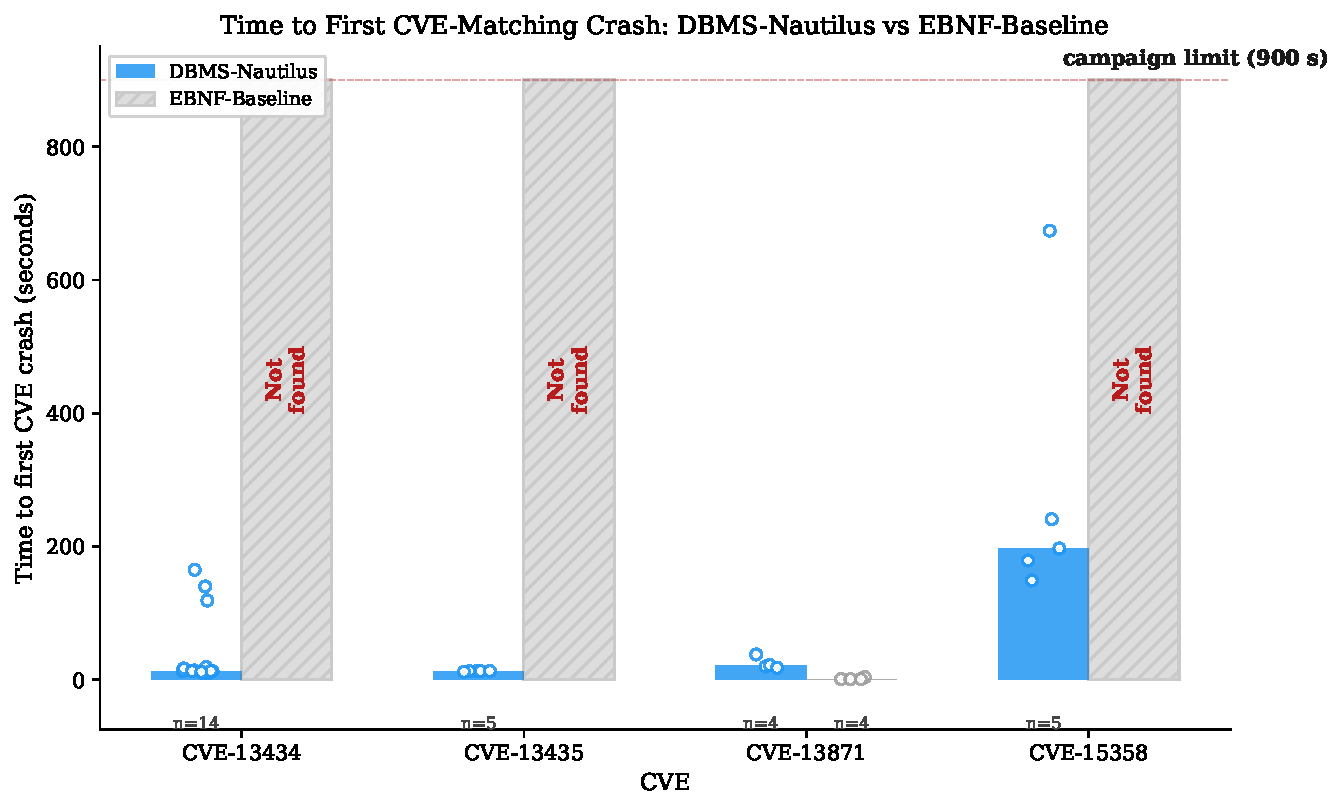
\includegraphics[width=\textwidth]{figures/fig_4_1_time_to_first_cve.pdf}
\caption{Time to first CVE-matching crash: DBMS-Nautilus vs EBNF-Baseline.}
\label{fig:time-to-cve}
\end{figure}

These results indicate that DBMS-Nautilus with seed rules achieves reliable CVE rediscovery for 4 of 4 target CVEs, with the majority of discoveries occurring within the first minutes of campaign execution.

\vspace{0.5em}
\noindent\fbox{\parbox{\dimexpr\linewidth-2\fboxsep-2\fboxrule}{%
\textbf{Answer to RQ1:} DBMS-Nautilus with seed rules reliably rediscovers 4 of 4 target CVEs (28/30 runs), with median time to first CVE crash ranging from 13\,s (CVE-2020-13435) to 197\,s (CVE-2020-15358). The EBNF-Baseline found only 1 of 4 CVEs (CVE-2020-13871), confirming that 3 of the 4 target vulnerabilities require domain-specific structural patterns that generic grammar specifications cannot express.}}
\vspace{0.5em}


\subsection{RQ2: Bug Detection}
\label{sec:rq2-results}

DBMS-Nautilus without seed rules discovers 13 distinct bug classes across 20 campaigns on 4 SQLite versions, producing 48 unique stack hashes after cross-campaign deduplication (individual campaigns produce many more hashes due to repeated discoveries; see RQ3 for per-campaign counts). The EBNF-Baseline discovers only 4 of the same 13 classes. Table~\ref{tab:rq2-comparison} compares the two grammars: for each bug class, it lists the versions on which each grammar triggered the bug and the number of unique stack hashes observed.

\begin{table}[htbp]
\caption{Bug classes discovered by each grammar.}
\label{tab:rq2-comparison}
\centering
\footnotesize
\setlength{\tabcolsep}{6pt}
\begin{tabular}{l >{\raggedright\arraybackslash}p{4.4cm} >{\raggedright\arraybackslash}p{2.5cm} >{\raggedright\arraybackslash}p{2.5cm} c}
\toprule
\textbf{Class} & \textbf{Bug Type} & \textbf{DBMS-Nautilus} & \textbf{EBNF-Baseline} & \textbf{Hashes} \\
\midrule
BC001 & Null ptr in \texttt{sqlite3\-Expr\-Code\-Target} & 3.30.1, 3.31.1, 3.32.0 & --- & 3 \\[1pt]
BC002 & Null ptr in \texttt{sqlite3\-Fts5\-Get\-Tokenizer} & 3.30.1, 3.31.1, 3.32.0, 3.32.2 & 3.30.1, 3.31.1, 3.32.0, 3.32.2 & 4/4 \\[1pt]
BC003 & Int overflow in \texttt{sqlite3\_str\_vappendf} & 3.30.1, 3.31.1, 3.32.0 & --- & 6 \\[1pt]
BC004 & Use-after-free in \texttt{Window\-Unlink\-From\-Select} & 3.30.1 & 3.30.1 & 1/1 \\[1pt]
BC005 & Float cast overflow in \texttt{alsoAnInt} & 3.31.1, 3.32.0, 3.32.2 & 3.30.1, 3.32.0 & 10/7 \\[1pt]
BC006 & Null ptr in \texttt{is\-Auxiliary\-Vtab\-Operator} & 3.31.1 & --- & 1 \\[1pt]
BC007 & Use-after-free in \texttt{reset\-Accumulator} & 3.30.1 & --- & 1 \\[1pt]
BC008 & Use-after-free in \texttt{sqlite3\-Expr\-Code\-Target} & 3.31.1 & --- & 13 \\[1pt]
BC009 & Float cast overflow in \texttt{Vdbe\-Mem\-Numerify} & 3.32.2 & --- & 2 \\[1pt]
BC010 & Null ptr in \texttt{sqlite3\-Select} & 3.31.1, 3.32.0 & --- & 2 \\[1pt]
BC011 & Heap use-after-free in \texttt{sqlite3\-Window\-List\-Delete} & 3.30.1 & 3.30.1 & 2/2 \\[1pt]
BC012 & Null ptr in \texttt{sqlite3\-Atoi64} & 3.30.1 & --- & 2 \\[1pt]
BC013 & Segfault in \texttt{sqlite3\-Expr\-Code\-Target} & 3.30.1 & --- & 1 \\
\midrule
\multicolumn{4}{l}{\textbf{Total: 13 classes (DBMS-Nautilus) vs 4 classes (EBNF-Baseline)}} & \textbf{48/14} \\
\bottomrule
\end{tabular}
\end{table}

The EBNF-Baseline's 4 classes (BC002, BC004, BC005, BC011) involve standard SQL constructs --- FTS virtual tables, window functions, and type casts --- that any comprehensive grammar exercises. The remaining 9 classes require domain-specific structural patterns absent from the EBNF grammar.

\begin{table}[htbp]
\caption{Bug classes per campaign by version.}
\label{tab:rq2-per-run}
\centering
\begin{tabular}{lcccc}
\toprule
\textbf{Grammar} & \textbf{3.30.1} & \textbf{3.31.1} & \textbf{3.32.0} & \textbf{3.32.2} \\
\midrule
\textbf{DBMS-Nautilus} & $\mathbf{7.0 \pm 1.0}$ & $\mathbf{6.0 \pm 0.7}$ & $\mathbf{4.4 \pm 0.5}$ & $\mathbf{2.4 \pm 0.9}$ \\
EBNF-Baseline & $2.8 \pm 0.8$ & $1.0 \pm 0.0$ & $1.2 \pm 0.5$ & $1.0 \pm 0.0$ \\
\midrule
\textbf{Ratio} & $2.5\times$ & $6.0\times$ & $3.7\times$ & $2.4\times$ \\
\bottomrule
\end{tabular}
\end{table}

Table~\ref{tab:rq2-per-run} breaks down the per-campaign discovery rate by version. DBMS-Nautilus finds $7.0 \pm 1.0$ bug classes per campaign on version~3.30.1 ($2.5\times$ more than the EBNF-Baseline's $2.8 \pm 0.8$), rising to $6.0\times$ on version~3.31.1 where the EBNF-Baseline finds only $1.0$ class per campaign. The advantage is smallest on version~3.32.2 ($2.4\times$), where fewer bugs remain after upstream fixes.

Four of the 13 bug classes match known CVEs by crash-line verification against the official proof-of-concept inputs: BC001 (CVE-2020-13435), BC003 (CVE-2020-13434), BC006 (CVE-2020-9327), and BC007 (CVE-2020-13871). These rediscoveries occurred without dedicated seed rules, confirming that the grammar's structural primitives can compositionally reconstruct CVE-triggering inputs. The remaining 9 classes have no CVE assignment; cross-version replay against 19 SQLite versions (3.26.0 through 3.53.0) on production (non-sanitizer) builds shows that 6 of them (BC004, BC008, BC010, BC011, BC012, BC013) cause segmentation faults across up to 10 consecutive releases.

\needspace{20\baselineskip}
\subsubsection{Selected Bugs}

Five representative bugs illustrate the kinds of defects that the grammar's structural compositions expose. The full list of 13 bug classes is summarized in Table~\ref{tab:rq2-comparison}.

\textbf{Null pointer in SELECT processing exposed by recursive CTE (BC010).} A recursive CTE combined with an \texttt{EXCEPT} operator and a window \texttt{FILTER} clause causes the query compiler to dereference a null \texttt{Table} pointer inside \texttt{sqlite3Select} (Listing~\ref{lst:bc010}). The grammar's \texttt{Recursive-CTE} and \texttt{Window-Func} non-terminals jointly produce this combination; neither construct appears in isolation in the EBNF-Baseline. The bug causes segmentation faults on production builds across six consecutive releases (3.30.0--3.32.2); no CVE was assigned. The EBNF-Baseline never triggered this path.

\begin{lstlisting}[caption={BC010: Null pointer in \texttt{sqlite3Select}.},label={lst:bc010},language=SQL,numbers=none]
-- Trigger SQL
WITH RECURSIVE a(x) AS (
  SELECT 1 UNION ALL SELECT x+1 FROM a WHERE x < 5
), b(y) AS (
  SELECT TRUE IN (VALUES (NULL)
    EXCEPT SELECT CURRENT_TIMESTAMP
    ORDER BY CURRENT_TIMESTAMP COLLATE NOCASE)
  FROM a
)
SELECT *, count(*) FILTER (WHERE RAISE(IGNORE))
  OVER (PARTITION BY RAISE(IGNORE)
        ORDER BY CURRENT_TIME DESC NULLS LAST
        ROWS BETWEEN CURRENT ROW AND UNBOUNDED FOLLOWING)
FROM b;

-- UBSan diagnostic
-- runtime error: member access within null pointer
--   of type 'Table' (aka 'struct Table')
-- in sqlite3Select
\end{lstlisting}

\textbf{Use-after-free with sanitizer blind spot (BC008).} A self-join with a correlated subquery combining \texttt{lead()} and \texttt{SUM()} triggers a misaligned memory access in the expression code generator (Listing~\ref{lst:bc008}). The misaligned address (\texttt{0x1ffffcaaaf0b}) confirms access to freed memory fill-pattern bytes. This bug exhibits a sanitizer blind spot on version~3.32.0: the ASan+UBSan build reports no error while the production build segfaults --- \texttt{SQLITE\_DEBUG} assertions mask the defect in instrumented builds. Affects 9 versions (3.26.0--3.32.0); fixed in 3.32.1. The 13 unique stack hashes reflect a rich space of triggering paths. The EBNF-Baseline cannot generate this self-join pattern.

\begin{lstlisting}[caption={BC008: Use-after-free in \texttt{sqlite3ExprCodeTarget}.},label={lst:bc008},language=SQL,numbers=none]
-- Trigger SQL
CREATE TABLE p(a UNIQUE);
SELECT p.a FROM p JOIN p q ON 3 = p.a
  NATURAL JOIN p
  WHERE p.a IN((
    SELECT(SELECT coalesce(lead(2) OVER(), SUM(a)))
    FROM p d WHERE p.a
  ));

-- UBSan diagnostic (3.31.1)
-- runtime error: member access within misaligned address
--   0x1ffffcaaaf0b for type 'struct AggInfo_func'
-- Stack: sqlite3ExprCodeTarget -> sqlite3ExprCodeExprList
--        -> innerLoopLoadRow -> selectInnerLoop
\end{lstlisting}

\textbf{Heap use-after-free in window list cleanup (BC011).} ASan confirms a heap-use-after-free in \texttt{sqlite3WindowListDelete} when a \texttt{Select} node whose window list was already deallocated is freed a second time (Listing~\ref{lst:bc011}). The trigger requires a \texttt{CHECK} constraint enclosing a window function inside a compound query --- a combination produced by the grammar's \texttt{Stress-Query} and \texttt{Validation-Op} non-terminals. Affects 3.26.0--3.30.1; fixed in 3.31.1. Both grammars found this bug, confirming that window functions are reachable through generic SQL.

\begin{lstlisting}[caption={BC011: Heap use-after-free in \texttt{sqlite3WindowListDelete}.},label={lst:bc011},language=SQL,numbers=none]
-- Trigger SQL
CREATE TABLE t3 (c1 TEXT CHECK ((SELECT * LIMIT EXISTS
  (SELECT * INTERSECT SELECT * FROM t1 WHERE CURRENT_DATE
   GROUP BY FALSE WINDOW w1 AS ()
   ORDER BY CURRENT_TIMESTAMP COLLATE NOCASE ASC),
  RAISE(IGNORE)))) WITHOUT ROWID;

-- ASan diagnostic
-- ERROR: AddressSanitizer: heap-use-after-free
-- READ of size 8 at 0xf531e6c029b8 thread T0
-- #0 sqlite3WindowListDelete -> clearSelect
--    -> sqlite3SelectDelete -> sqlite3ExprDeleteNN
\end{lstlisting}

\textbf{CVE-2020-9327 rediscovery via generated column composition (BC006).} The query planner dereferences a null \texttt{Table} pointer when classifying operators for a view that references a generated column with a \texttt{UNIQUE} constraint (Listing~\ref{lst:bc006}). Rediscovering this CVE requires four structural elements from different grammar groups --- \texttt{GENERATED ALWAYS AS}, \texttt{UNIQUE}, \texttt{CREATE VIEW}, and a multi-table join --- produced jointly by the grammar's \texttt{Schema-Setup} and \texttt{Stress-Query} non-terminals. Affects 3.31.1 only; fixed in 3.32.0. The EBNF-Baseline has no generated column rules and cannot reach this path.

\begin{lstlisting}[caption={BC006: Null pointer in \texttt{isAuxiliaryVtabOperator} (CVE-2020-9327).},label={lst:bc006},language=SQL,numbers=none]
-- Trigger SQL
CREATE TABLE v0(v3, v1 GENERATED ALWAYS AS (v3) UNIQUE);
CREATE TABLE v5(v6 UNIQUE, v7 UNIQUE);
CREATE VIEW v8 AS
  SELECT coalesce(v3, v1) AS v9 FROM v0 WHERE v1 IN('');
SELECT * FROM v8 JOIN v5 WHERE 0 > v7 AND v9 OR v6 = ' ';

-- UBSan diagnostic
-- runtime error: member access within null pointer
--   of type 'Table' (aka 'struct Table')
-- Stack: isAuxiliaryVtabOperator -> exprAnalyze
--        -> sqlite3WhereExprAnalyze -> sqlite3WhereBegin
\end{lstlisting}

\textbf{Use-after-free in window function unlinking (BC004).} A view definition combined with an \texttt{ORDER BY} clause inside a compound query triggers a store to a misaligned address during window function cleanup (Listing~\ref{lst:bc004}). The address \texttt{0xaaaaaaaaaaaaaaaa} is the \texttt{SQLITE\_DEBUG} freed-memory fill pattern, confirming that the code writes through a dangling pointer. The resulting segfault is non-deterministic on production builds. Affects 3.30.0--3.30.1; fixed in 3.31.1. Both grammars found this bug, indicating that view-plus-window combinations are exercised even by generic SQL generation.

\begin{lstlisting}[caption={BC004: Use-after-free in \texttt{sqlite3WindowUnlinkFromSelect}.},label={lst:bc004},language=SQL,numbers=none]
-- Trigger SQL
CREATE TABLE IF NOT EXISTS p(a INTEGER);
CREATE TABLE IF NOT EXISTS q(b INTEGER);
CREATE VIEW IF NOT EXISTS vp AS SELECT a FROM p ORDER BY a;
SELECT (SELECT t2.* FROM r NOT INDEXED WHERE FALSE COLLATE
  RTRIM UNION SELECT FALSE FROM t1 WHERE CURRENT_TIME
  COLLATE RTRIM GROUP BY TRUE NOT NULL HAVING NULL
  WINDOW w1 AS (PARTITION BY CURRENT_TIME)
  ORDER BY quote(CURRENT_DATE COLLATE RTRIM GLOB FALSE
  COLLATE NOCASE >= TRUE) DESC NULLS LAST)
  AS z39y_3sry46f___gb75,
  FALSE COLLATE BINARY AS gu571__i14_6_d_3f1_9__o
FROM p, q
WHERE p.a = (SELECT 0 INTERSECT SELECT b FROM vp)
  AND p.a = 0;

-- UBSan diagnostic
-- runtime error: store to misaligned address
--   0xaaaaaaaaaaaaaaaa for type 'Window *'
--   (requires 8 byte alignment) -- freed memory pattern
-- in sqlite3WindowUnlinkFromSelect
\end{lstlisting}

\vspace{0.5em}
\noindent\fbox{\parbox{\dimexpr\linewidth-2\fboxsep-2\fboxrule}{%
\textbf{Answer to RQ2:} DBMS-Nautilus discovers 13 bug classes (48 hashes) without seed rules, including 4 CVE rediscoveries and 6 non-CVE bugs that cause segmentation faults on production builds across up to 10 consecutive releases. The EBNF-Baseline finds 4 of the 13 classes (14 hashes); 9 bug classes are exclusive to DBMS-Nautilus.}}
\vspace{0.5em}


\subsection{RQ3: Performance Trade-off}
\label{sec:rq3-results}

DBMS-Nautilus and the EBNF-Baseline were compared across four metrics using the Mann-Whitney~$U$ test with Cliff's~$d$ effect size (Table~\ref{tab:rq3-stats}). Each cell reports mean $\pm$ standard deviation; $n=5$ per cell except EBNF-Baseline 3.32.0 where $n=4$.

\begin{table}[htbp]
\caption{Statistical comparison: DBMS-Nautilus vs EBNF-Baseline.}
\label{tab:rq3-stats}
\centering
\resizebox{\textwidth}{!}{%
\begin{tabular}{llrrrl}
\toprule
\textbf{Metric} & \textbf{Version} & \textbf{DBMS-Nautilus} & \textbf{EBNF-Baseline} & \textbf{$p$-value} & \textbf{Cliff's $d$} \\
\midrule
\multirow{4}{*}{Unique RCs}
  & 3.30.1 & $\mathbf{215.4 \pm 24.4}$ & $3.6 \pm 2.1$ & 0.012 & $+1.00$ (large) \\
  & 3.31.1 & $\mathbf{170.6 \pm 72.4}$ & $1.0 \pm 0.0$ & 0.007 & $+1.00$ (large) \\
  & 3.32.0 & $\mathbf{139.4 \pm 73.0}$ & $2.0 \pm 2.0$ & 0.018 & $+1.00$ (large) \\
  & 3.32.2 & $\mathbf{296.8 \pm 38.2}$ & $1.0 \pm 0.0$ & 0.007 & $+1.00$ (large) \\
\midrule
\multirow{4}{*}{Edge Cov.}
  & 3.30.1 & $19{,}862 \pm 274$ & $\mathbf{23{,}323 \pm 152}$ & 0.008 & $-1.00$ (large) \\
  & 3.31.1 & $20{,}010 \pm 915$ & $\mathbf{23{,}182 \pm 341}$ & 0.008 & $-1.00$ (large) \\
  & 3.32.0 & $20{,}017 \pm 1{,}109$ & $\mathbf{23{,}645 \pm 300}$ & 0.016 & $-1.00$ (large) \\
  & 3.32.2 & $20{,}838 \pm 177$ & $\mathbf{23{,}811 \pm 166}$ & 0.008 & $-1.00$ (large) \\
\midrule
\multirow{4}{*}{Throughput}
  & 3.30.1 & $90.7 \pm 7.1$ & $\mathbf{196.3 \pm 15.9}$ & 0.008 & $-1.00$ (large) \\
  & 3.31.1 & $92.6 \pm 14.1$ & $\mathbf{182.7 \pm 12.2}$ & 0.008 & $-1.00$ (large) \\
  & 3.32.0 & $84.9 \pm 10.8$ & $\mathbf{198.0 \pm 11.8}$ & 0.016 & $-1.00$ (large) \\
  & 3.32.2 & $95.2 \pm 9.3$ & $\mathbf{182.4 \pm 15.8}$ & 0.008 & $-1.00$ (large) \\
\midrule
\multirow{4}{*}{TTFC (s)}
  & 3.30.1 & $1.8 \pm 0.8$ & $1.8 \pm 1.3$ & 0.821 & $+0.12$ (negl.) \\
  & 3.31.1 & $1.8 \pm 0.4$ & $\mathbf{1.2 \pm 0.4}$ & 0.093 & $+0.60$ (large) \\
  & 3.32.0 & $1.6 \pm 0.9$ & $\mathbf{1.0 \pm 0.0}$ & 0.240 & $+0.40$ (medium) \\
  & 3.32.2 & $2.0 \pm 0.7$ & $\mathbf{1.8 \pm 1.1}$ & 0.740 & $+0.16$ (small) \\
\bottomrule
\end{tabular}}
\end{table}

The results reveal a clear trade-off between structural complexity and raw throughput. The EBNF-Baseline achieves $1.9\times$--$2.3\times$ higher throughput (mean 189.9 executions per second vs 90.8 for DBMS-Nautilus) and $1.1\times$--$1.2\times$ higher edge coverage (mean 23{,}490 vs 20{,}182 edges). However, DBMS-Nautilus discovers $60\times$--$297\times$ more unique root causes per campaign (mean 205.6 vs 1.9), with large effect sizes ($d = 1.00$, $p < 0.05$) on all four versions.

Time to first crash (TTFC) shows no statistically significant difference between the two grammars on any version ($p > 0.05$ on all four), indicating that both grammars find their first crash within seconds of campaign start. The throughput disadvantage of DBMS-Nautilus does not translate into a delay in initial crash discovery.

Figure~\ref{fig:coverage-growth} shows the edge coverage growth over the 15-minute campaign duration for both grammars. The EBNF-Baseline reaches higher absolute coverage due to its higher throughput and broader syntactic variety, but DBMS-Nautilus's coverage growth rate suggests that it explores a smaller but more crash-producing subset of the code.

\begin{figure}[htbp]
\centering
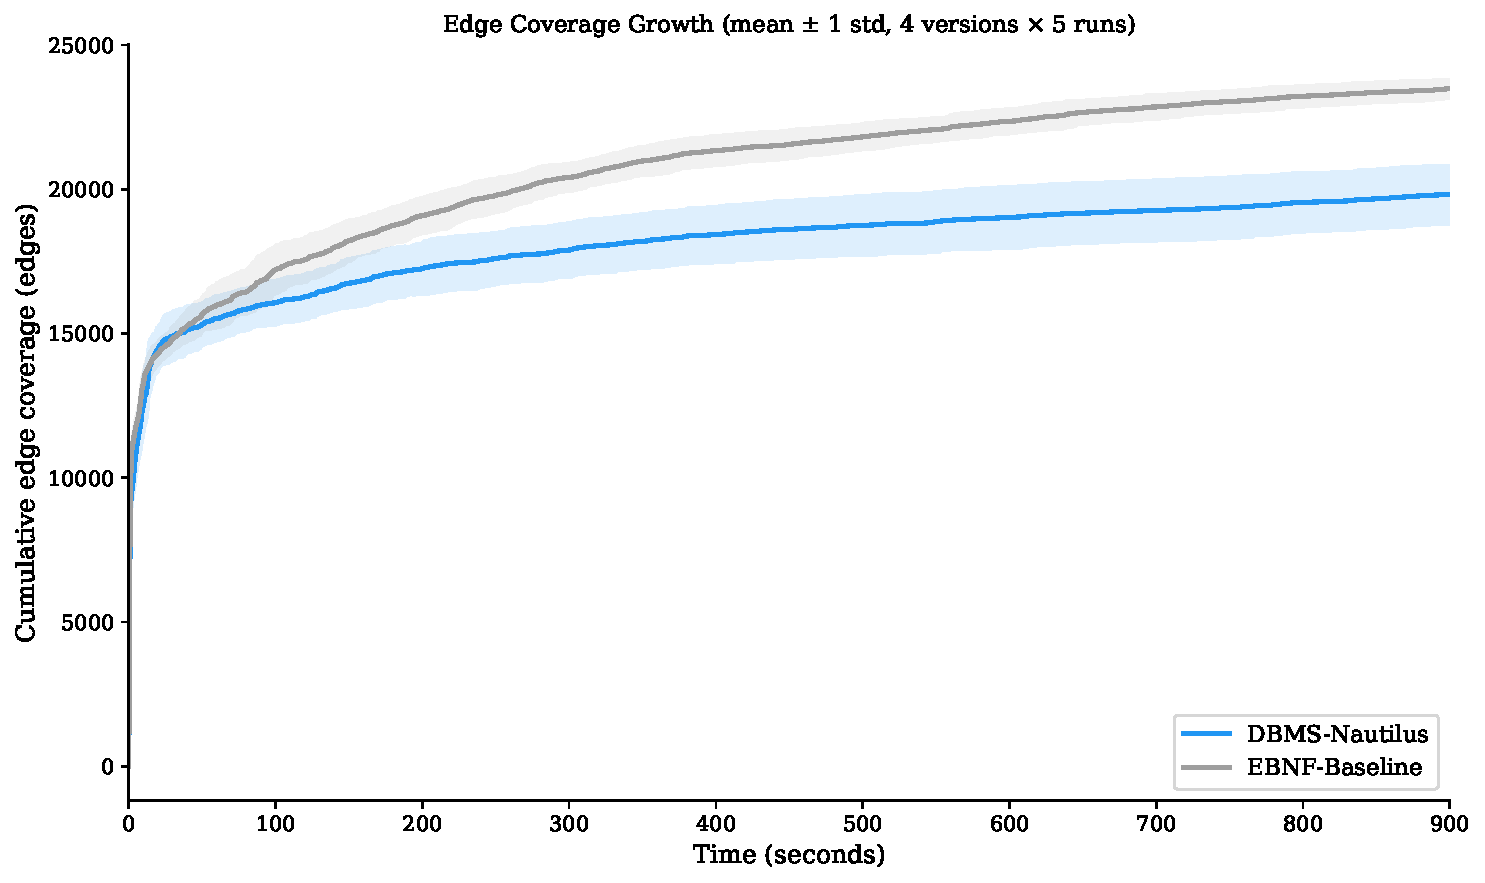
\includegraphics[width=\textwidth]{figures/fig_4_3_coverage_growth.pdf}
\caption{Edge coverage growth over time.}
\label{fig:coverage-growth}
\end{figure}

The EBNF-Baseline's simpler production rules generate shorter SQL inputs, yielding faster execution per test case; Figure~\ref{fig:throughput} shows throughput across all four versions.

\begin{figure}[htbp]
\centering
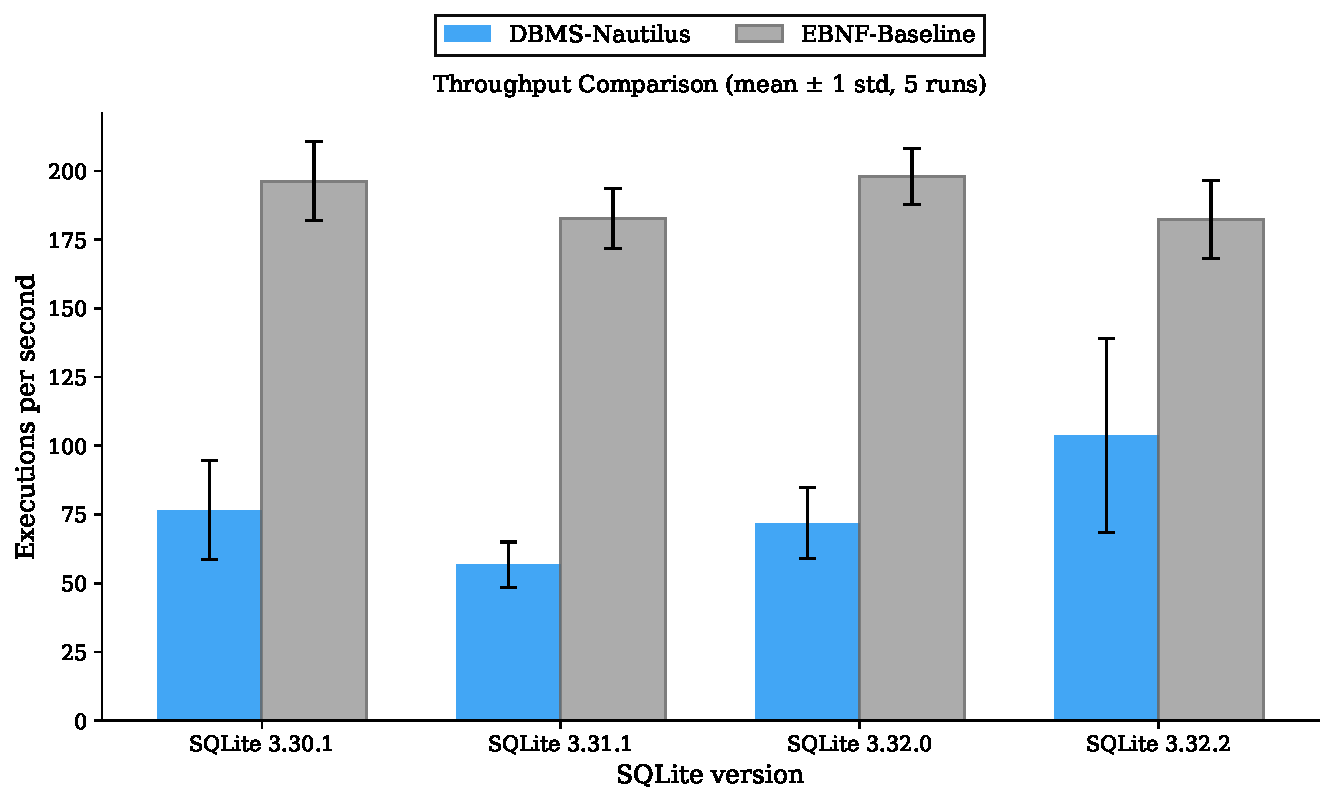
\includegraphics[width=\textwidth]{figures/fig_4_4_throughput.pdf}
\caption{Throughput comparison across SQLite versions.}
\label{fig:throughput}
\end{figure}

Figure~\ref{fig:ttfc} shows the time-to-first-crash distribution; both grammars find their first crash within seconds on every version, confirming that the throughput gap does not delay initial crash discovery.

\begin{figure}[htbp]
\centering
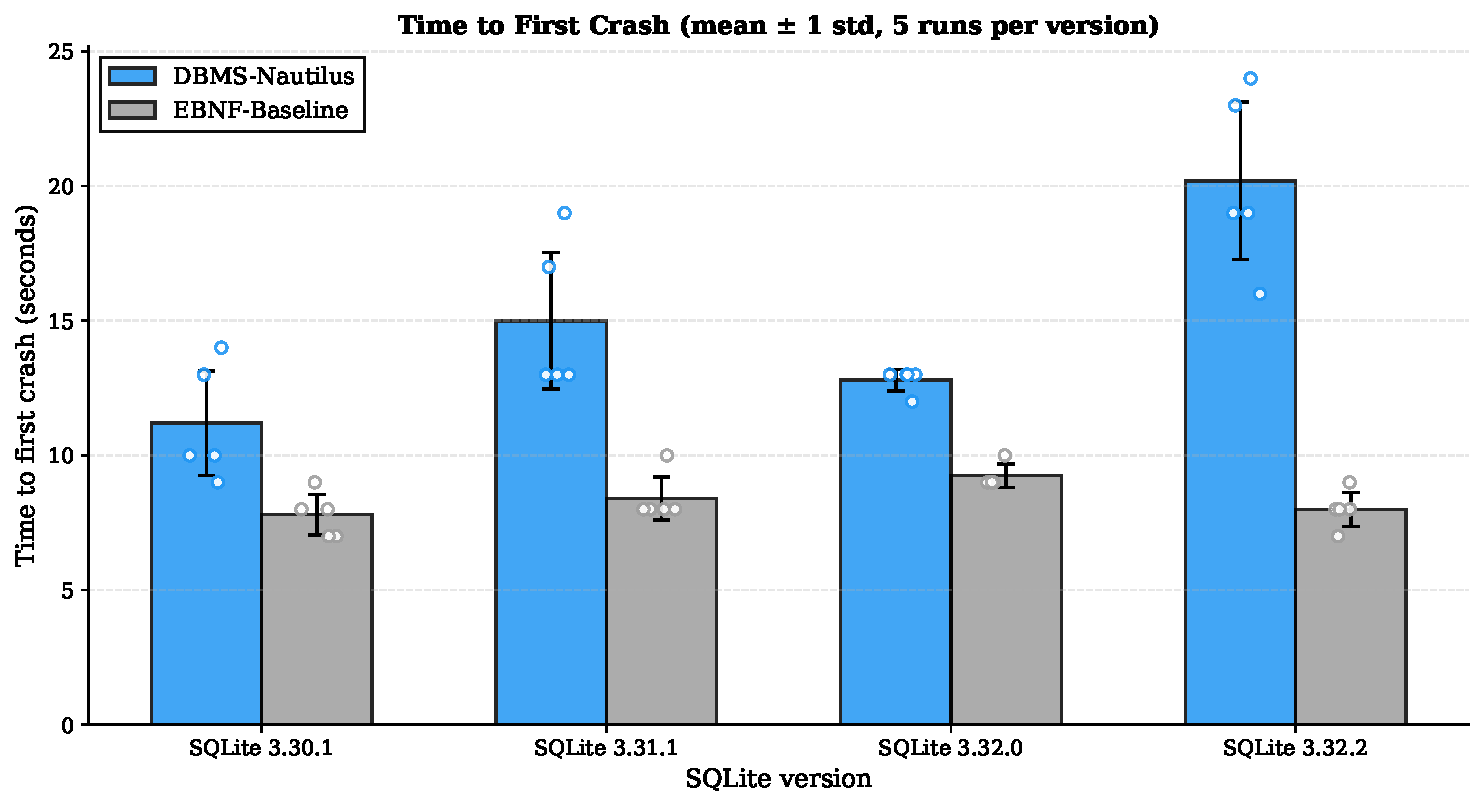
\includegraphics[width=\textwidth]{figures/fig_4_5_time_to_first_crash.pdf}
\caption{Time to first UBSan/ASan crash (excluding debug assertions).}
\label{fig:ttfc}
\end{figure}

DBMS-Nautilus sacrifices throughput and edge coverage breadth in exchange for higher crash diversity: structural complexity in grammar design redirects fuzzing effort toward code paths that produce crashes, at the cost of raw execution speed.

\vspace{0.5em}
\noindent\fbox{\parbox{\dimexpr\linewidth-2\fboxsep-2\fboxrule}{%
\textbf{Answer to RQ3:} DBMS-Nautilus discovers $108\times$ more unique root causes per campaign (205.6 vs 1.9) at the cost of 52.1\% lower throughput and 14.1\% lower edge coverage. The throughput reduction does not delay initial crash discovery: time to first crash shows no statistically significant difference between the two grammars ($p > 0.05$ on all versions). The EBNF-Baseline's higher coverage is shallow --- it executes more inputs but the additional coverage does not translate into proportional crash discovery.}}
\vspace{0.5em}


\section{Discussion}
\label{sec:discussion}

\subsection{Qualitative Analysis}
\label{sec:qualitative}

The 13 bug classes discovered by DBMS-Nautilus (RQ2) were validated through cross-version testing against 19 SQLite releases (3.26.0 through 3.53.0) using both sanitizer-instrumented and production (no-sanitizer) harness builds.

\emph{CVE-matching bugs} (4 classes, 30.8\% of total). BC001 (CVE-2020-13435), BC003 (CVE-2020-13434), BC006 (CVE-2020-9327), and BC007 (CVE-2020-13871) are rediscoveries of known CVEs through compositional generation without seed rules. These validate the grammar's primary design objective: encoding crash-producing patterns that can reconstruct CVE-triggering inputs without embedding proof-of-concept strings. For BC001, the grammar's join and window function patterns trigger a null pointer dereference in the expression code generator, matching CVE-2020-13435. For BC003, the \texttt{Boundary-Func-Call} non-terminal produces a \texttt{printf} call with \texttt{INT\_MAX} precision, matching CVE-2020-13434. For BC006, the combination of generated column, \texttt{UNIQUE} constraint, view, and join matches CVE-2020-9327. For BC007, the combination of window function, aggregate, and \texttt{EXCEPT} compound operator triggers a use-after-free in \texttt{resetAccumulator}, matching CVE-2020-13871.

\emph{Non-CVE production bugs} (6 classes, 46.2\% of total). BC004, BC008, BC010, BC011, BC012, and BC013 cause segmentation faults on production builds and were fixed between versions 3.31.1 and 3.32.3 without CVE assignment. BC008 and BC013 each affect 9--10 consecutive SQLite versions. BC010 affects 6 versions (3.30.0--3.32.2). BC008 exhibits a sanitizer blind spot on version~3.32.0: the ASan+UBSan build reports no error while the production build segfaults.

\emph{Sanitizer-only bugs} (3 classes, 23.1\% of total). BC002, BC005, and BC009 trigger UBSan diagnostics but do not crash production builds on x86\_64. BC002 (FTS5 tokenizer null pointer) persists across 15 versions until 3.36.0.

\subsection{Failure Cases and Limitations}
\label{sec:limitations}

At least two concrete limitations of the proposed approach were identified during the evaluation:

\begin{enumerate}
  \item \textbf{Context-free grammar cannot enforce semantic validity.} The grammar is context-free and cannot enforce type correctness, referential integrity, or valid column count matching between \texttt{INSERT} values and table definitions. Semantically invalid SQL statements are generated and immediately rejected by SQLite's parser or query planner, consuming execution time without contributing to coverage. The throughput gap between DBMS-Nautilus (90.8 execs/sec) and the EBNF-Baseline (189.9 execs/sec) is partially attributable to DBMS-Nautilus generating longer, more complex inputs that take more time to parse and reject.

  \item \textbf{Manual CVE analysis dependency.} The DBMS-Nautilus methodology requires manual expertise to identify which SQL constructs are relevant to each vulnerability. The effectiveness of the approach depends on the quality of this analysis: if a critical structural pattern is missed or incorrectly characterized, the corresponding grammar rules will be absent or ineffective. Automating this analysis --- for example, through differential code analysis between patched and unpatched versions --- is an open research question.
\end{enumerate}

\subsection{Threats to Validity}
\label{sec:threats}

\paragraph{Internal validity.}
Stack-hash deduplication using the top 5 frames is a heuristic that may both over-count and under-count bug classes. Over-counting occurs when two manifestations of the same root cause crash through different call paths; under-counting occurs when distinct bugs crash through the same 5-frame sequence. The \texttt{SQLITE\_DEBUG} build flag introduces an additional confound: it fills freed memory with \texttt{0xAA} bytes, causing use-after-free bugs to manifest as misaligned-access diagnostics rather than heap-use-after-free reports. This was addressed through no-debug harness replay for CVE confirmation (see Table~\ref{tab:cve-rediscovery}), but may affect the classification accuracy of non-CVE bug classes. Campaign durations of 15~minutes may miss bugs requiring longer exploration or rarer compositional combinations; however, extending campaigns introduces diminishing returns in coverage-guided fuzzing.

\paragraph{External validity.}
All experiments target a single DBMS --- SQLite~\citep{sqlite} --- with a single input language (SQL). SQLite is an embedded database with a compact codebase (${\sim}$150{,}000 lines of C), and its bug landscape may not be representative of larger server-based systems such as MySQL or PostgreSQL. The comparison uses a single baseline grammar (EBNF-Baseline) rather than multiple baselines or existing fuzzing tools such as SQLsmith~\citep{sqlsmith} or Squirrel~\citep{squirrel}. Direct comparison with these tools was not feasible because they use fundamentally different fuzzing strategies (query-plan-guided generation for SQLsmith, AST-level mutation for Squirrel) that cannot be isolated to a grammar-only comparison. The EBNF-Baseline isolates the effect of grammar design by holding all other variables constant.

\paragraph{Construct validity.}
The 80\% fidelity threshold for CVE signature matching is an arbitrary cutoff. A higher threshold would reduce false positive matches but might miss legitimate rediscoveries where the stack trace differs due to compiler optimizations or ASan instrumentation overhead. The sanitizer oracle misses entire categories of bugs: logic bugs producing incorrect results without undefined behavior, and denial-of-service bugs causing non-termination without crashing. Edge coverage as measured by the AFL-style bitmap is subject to hash collisions, where distinct edges map to the same bitmap byte, potentially causing the fuzzer to miss coverage-increasing inputs.

\subsection{Summary}
\label{sec:summary}

The experimental evaluation demonstrates three principal findings. First, DBMS-Nautilus with seed rules reliably rediscovers 4 out of 4 target CVEs across 20 campaigns, supporting the hypothesis that domain-knowledge-driven grammar engineering can reconstruct CVE-triggering inputs from independently encoded structural primitives (RQ1). Second, DBMS-Nautilus without seed rules discovers 13 distinct bug classes (48 unique hashes), validated through cross-version testing against 19 SQLite releases: 4 are CVE rediscoveries, 6 are non-CVE production bugs affecting up to 10 consecutive releases each, and 3 are sanitizer-only detections (RQ2). Nine of the 13 bug classes were found exclusively by DBMS-Nautilus. Third, DBMS-Nautilus sacrifices throughput ($2.1\times$ slower) and edge coverage (14.1\% lower) in exchange for $108\times$ more unique root causes per campaign, indicating that structural complexity redirects fuzzing effort toward crash-producing code at the cost of raw execution speed (RQ3). The EBNF-Baseline found 4 of the 13 bug classes (BC002, BC004, BC005, BC011), none of which match the 4 CVE-rediscovery classes.
